\noindent
{\Large \textbf{\section{Аналитика}}} \par
\vspace{-20pt}

{\Large \textbf{\subsection{Описание предметной области}}} \par

Предметная область охватывает организацию выставочной деятельности музея. Исторический музей - это культурно-просветительское и научно-иссле-\\довательское учреждение, которое занимается сбором, изучением, реставрацией и демонстрацией различных предметов, имеющих культурно-историческую ценность. Эта ценность определяется историками - людьми, профессионально занимающимися изучением и описанием прошлого человеческого общества, основываясь на различных материальных и нематериальных источниках. К материальным источникам можно отнести различные документы и предметы, созданные в рассматриваемые периоды истории, к нематериальным - устное народное творчество, легенды и предания. Ценность предметов может оцениваться по-разному, это зависит от временного промежутка, в который они были созданы, материалов, уникальности, религиозной и культурной значимости для определенных сообществ. \par

Фонды музея - это совокупность всех материалов, которые в соответствии с установленными правилами были приняты музеем на постоянное хранение \cite{site:sources1}. При этом, они могут храниться непосредственно в фондохранилище или находиться на экспозиции. Фондохранилище - это пространство в музее, предназначенное для хранения предметов коллекции, не находящихся на экспозиции. В этом помещении (помещениях) каждый предмет хранится в соответствии с требуемыми условиями хранения, которые включают определенный уровень влажности, температуры и освещенности. \par

За сохранность фондов отвечает хранитель фондов - это специалист, который несёт персональную ответственность за сохранность, учёт, научное описание и движение музейных предметов, закреплённых за фондами музея. Его обязанностями являются, инвентаризация, паспортизация, научное описание предметов, контроль условий хранения, контроль транспортировки предметов на выставки и реставрации, содействие работе исследователей и кураторов выставок. \par

В соответствии со значением предметов для науки и культуры, музейные фонды делятся на основной фонд и фонд научно-вспомогательных материалов. Научно-вспомогательный фонд формируется из предметов, выполняющих вспомогательную функцию, то есть научно-вспомогательных материалов. Научно-вспомогательные материалы – это предметы, помогающие в изучении других экспонатов. К ним относят экспозиционные научно-вспомогательные материалы (муляжи, копии, макеты, модели, реконструкции, планы). По своим функциям научно-вспомогательные материалы помогают представить внешний облик предмета в случае его отсутствия в музее, или в целях его сохранности (копии, муляжи), помогают уяснить строение предмета (схемы машин, механизмов), показывают связи экспонатов с историческими событиями (диаграммы, карты-схемы). Кроме того, к ним относят предметы очень плохой сохранности, которые не отвечают критериям отбора в основной фонд \cite{site:sources2}. \par

Основной фонд музея состоит из подлинных предметов. Это могут быть предметы быта и одежды, драгоценности, оружие и доспехи, карты, договоры, документы, письма, картины и гравюры, статуи, различные религиозные элементы, мебель, технические устройства, транспортные средства. Для каждого объекта хранителем фондов составляется паспорт, который заполняется данными о хронологических рамках создания, материалах, размерах, весе, принадлежности к определенной коллекции (предметам, выделенным историками в определенную группу по общности некоторых временн\'{ы}х или культурных признаков) и условиях хранения. \par

В фондах музея также работают реставраторы - специалисты, которые занимаются сохранением, консервацией и восстановлением музейных предметов. Деятельность этих работников тесно связана с хранителем фондов, потому что именно от него им поступают задачи по оценке состояния экспонатов, в том числе для последующей реставрации (процесса возвращения вещи первоначального состояния). Кроме того, реставраторы определяют условия хранения предметов в фондохранилище и передают эту информацию хранителю фондов. \par

Куратор выставок занимается разработкой новых выставок на территории музея. Выставка представляет собой организованную демонстрацию предметов из музейных фондов, объединённых общей темой и концепцией. Деятельность куратора заключается в разработке идей и концепций экспозиций, определении актуальности выбранной тематики, проектировании архитектуры выставочного пространства, реализации образовательных программ. На выставках демонстрируется ограниченная часть музейных фондов, поскольку не все экспонаты могут быть представлены публике из-за необходимости соблюдения определенных условий хранения, а иногда и потребности в реставрационных работах. \par

Всего выделяют шесть основных типов современных музейных экспозиций: созерцательный, тематический, средовой, систематический, интерактивный и прикладной. Созерцательный тип предполагает предъявление предметов преимущественно в эстетическом ключе с акцентом на эмоциональное восприятие. Тематический тип строится на включении экспонатов в более широкий исторический, социальный или культурный контекст с использованием пояснительных материалов. Средовой тип ориентирован на воссоздание атмосферы времени и пространства, в которых существовали представленные объекты. Систематический тип основывается на упорядоченном, классификационном показе собрания, нередко в формате открытого хранения с расширенной информацией. Интерактивный тип предполагает активное вовлечение посетителя в процесс познания через диалоговые и мультимедийные средства. Прикладной тип предоставляет возможность непосредственного практического взаимодействия с объектами и получения личного опыта \cite{site:sources3}. \par

Подготовка любой выставки проходит через определенную последовательность этапов. Первым идет разработка концепции. Куратор предлагает идею, учитывая научный интерес и предпочтения публики, определяет цели и задачи будущего проекта. После этого требуется отбор произведений, который происходит при работе с предметами в фондохранилище. После примерного отбора экспонатов следует согласование концепции и состава выставки с экспертами-историками и хранителем фондов. При этом необходимо, чтобы тема и концепция соответствовали стратегии выставочной работы музея на ближайшие годы. Далее следует создание заявки на выставку и составление подробной сметы расходов. После этого заявка со сметой рассматриваются директором музея. Раз в год все одобренные директором выставочные заявки отправляют в Министерство культуры, где специальная комиссия определяет, какие проекты будут поддержаны, а какие будут ждать своей очереди. \par

Если выставочный проект одобрен, то для выставки находят организатора, который занимается реализацией планов куратора.  Для этого определяется место проведения и утверждаются точные даты экспонирования, утверждается финансирование определённых закупок и услуг, необходимых для создания и проведения выставки. После согласования статей расходов начинается самый насыщенный этап - поиск исполнителей и заключение контрактов, закупка, организация транспортировки, работа над дизайном экспозиции, подготовка сопроводительных материалов, аннотаций, программы мероприятий, запуск PR-кампании выставки, освещение в СМИ и социальных сетях. Завершается подготовка монтажом выставки, который чаще всего длится 3-4 дня и включает в себя расположение экспонатов в соответствии с экспозиционным планом, оформление зала, настройку света. Этот долгий путь завершается вернисажем выставки (вернисаж - это торжественное открытие выставки, на котором присутствуют приглашенные персоны и СМИ) \cite{site:sources4}. \par


%\vspace{-10pt}
{\Large \textbf{\subsection{Цели функционирования базы данных}}} \par

\begin{enumerate}
    \item Ведение централизованного реестра музейных предметов.
    \item Ведение реестра проводимых в музее выставок.
    \item Хранение планов размещения выставок в залах музея.
\end{enumerate}


\vspace{-40pt}
{\Large \textbf{\subsection{Перечень сущностей и их атрибутов}}} \par


\begin{enumerate}
    \item \textbf{Сотрудник} - учетная запись специалиста музея, определяющая его полномочия и зону ответственности в работе с фондами или при организации выставок.
    \begin{itemize}
        \item Фамилия.
        \item Имя.
        \item Отчество.
        \item Должность (куратор, организатор, хранитель, реставратор).
        \item Номер телефона.
    \end{itemize}

    \item \textbf{Фонд} - полное собрание музейных предметов, прошедших научный отбор и принятых музеем на постоянное хранение в соответствии с установленными правилами содержания.
    \begin{itemize}
        \item Тип фонда (основной, вспомогательный).
        \item Принадлежность к коллекции (Пример: <<Ближневосточные монеты периода высокого средневековья>>).
        \item Уровень доступа.
        \item Ответственный хранитель.
    \end{itemize}

    \item \textbf{Фондохранилище} - специализированное помещение, оборудованное для долгосрочного хранения предметов коллекции, не задействованных в текущих экспозициях музея.
    \begin{itemize}
        \item Вместимость (максимальное количество объектов для размещения).
        \item Температура.
        \item Влажность.
        \item Освещенность.
    \end{itemize}

    \item \textbf{Экспонат} - предмет, который обладает культурной и научной ценностью, а также числится на хранении в фонде музея с целью изучения или участия в выставках. 
    \begin{itemize}
        \item Инвентарный номер.
        \item Название.
        \item Текущий статус (в хранилище, на экспозиции, на реставрации).
        \item Принадлежность к коллекции.
    \end{itemize}

    \item \textbf{Технический паспорт} - документ, приписанный к определенному экспонату из фондов музея, который содержит информацию о его характеристиках, состоянии и условиях содержания.
    \begin{itemize}
        \item Состояние (заключение реставратора о физической сохранности).
        \item Тип экспоната (оружие, одежда, документ, монета и др.).
        \item Вес.
        \item Эпоха.
        \item Материал.
        \item Требуемая влажность.
        \item Требуемая температура.
        \item Требуемая освещенность.
    \end{itemize}

    \item \textbf{Выставка} - временная тематическая демонстрация группы экспонатов, объединенных общей концепцией и определенными сроками показа посетителям музея.
    \begin{itemize}
        \item Название.
        \item Тема.
        \item Тип.
        \item Состояние (подбор экспонатов, согласование, организация пространства, действующая)
        \item Ответственный куратор.
    \end{itemize}

    \item \textbf{Экспозиционный план} - документ, фиксирующий перечень задействованных в выставке предметов и их размещение в выставочном пространстве.
    \begin{itemize}
        \item Версия плана (черновик, окончательная).
        \item Ответственный организатор.
        \item Необходимое количество витрин.
        \item Логика осмотра (хронологическая, тематическая, свободная).
        \item Концепция взаимодействия (атмосферная, интерактивная, традиционная выставка)
        
    \end{itemize}

    \item \textbf{Витрина} - специализированное выставочное оборудование, расположенное в залах музея и предназначенное для демонстрации экспонатов посетителям.
    \begin{itemize}
        \item Уровень освещенности.
        \item Поддерживаемая влажность.
        \item Поддерживаемая температура.
    \end{itemize}

    \item \textbf{Смета расходов} - финансовый документ, отражающий планируемые затраты на услуги логистики, страховки, монтажа, необходимые для реализации проекта выставки.
    \begin{itemize}
        \item Расходы на рекламу.
        \item Расходы на реставрацию.
        \item Расходы на создание сопровождающих материалов.
        \item Расходы на услуги наемных рабочих.
        \item Статус согласования.
    \end{itemize}

    \item \textbf{Выставочное пространство} - оборудованный зал или территория музея, предназначенная для публичного показа экспонатов, условия содержания которых подходят для данного пространства.
    \begin{itemize}
        \item Тип помещения (кабинет, арсенал, коридор).
        \item Вместимость посетителей.
        \item Уровень естественной освещенности.
        \item Уровень охраны.
    \end{itemize}
\end{enumerate}

\vspace{-40pt}
{\Large \textbf{\subsection{Перечень ролей}}} \par

\begin{enumerate}
    \item \textbf{Куратор выставок} — профессионал, разрабатывающий научную концепцию и тему выставки, а также осуществляющий подбор экспонатов из фондов музея и определяющий их роль в рамках конкретного выставочного проекта.
    \item \textbf{Организатор выставок} — специалист, отвечающий за техническую реализацию выставки, координацию логистики, закупок, монтажа экспозиции, а также ответственный за финансовый контроль утвержденной сметы расходов.
    \item \textbf{Хранитель фондов} - специалист, который несёт ответственность за сохранность, учёт, научное описание и движение музейных предметов, закреплённых за фондами музея.
    \item \textbf{Реставратор} — эксперт, занимающийся оценкой физического состояния предметов, проведением работ по их восстановлению и консервации, а также устанавливающий допустимые параметры среды для безопасного экспонирования.
\end{enumerate}

\vspace{-40pt}
{\Large \textbf{\subsection{ER-диаграмма и схема связи объектов}}} \par

ER-диаграмма с текстом ее чтения представлена на Рис.\ref{ER}. \par
Ниже выделен текст чтения ER-диаграммы.
\vspace{4pt}
\begin{enumerate}[noitemsep, topsep=0pt]
    \item Сотрудник занимает должность.
    \item Должность наделяет полномочиями.
    \item Полномочия заведовать фондом.
    \item Полномочия реставрировать экспонаты.
    \item Полномочия составлять технические паспорта.
    \item Полномочия курировать выставки.
    \item Полномочия составлять смету расходов.
    \item Фонд располагает коллекциями.
    \item Коллекция объединяет экспонаты. 
    \item Экспонат закреплен за фондохранилищем.
    \item Экспонат сопровождается техническим паспортом.
    \item Выставка реализуется по экспозиционному плану.
    \item Экспозиционный план обосновывает смету расходов.
    \item Экспозиционный план характеризует выставочное пространство.
    \item Выставочное пространство располагает местами экспонирования.
    \item Место экспонирования демонстрирует экспонат.
\end{enumerate}

\storeareas\MySavedValues 

% 2. Меняем формат на A3 и ориентацию на альбомную
% Важно: \clearpage обязателен перед сменой формата
%\clearpage
\KOMAoptions{
    paper=a3, 
    paper=landscape, 
    DIV=15,           % Делаем поля поменьше, так как на A3 их стандартный размер огромен
    BCOR=0mm,         % Убираем отступ под переплет для этого листа
    pagesize          % Гарантируем, что PDF поймет смену размера
}
\recalctypearea

\noindent
%\vspace{20pt}
\begin{figure}[H]
    \centering
    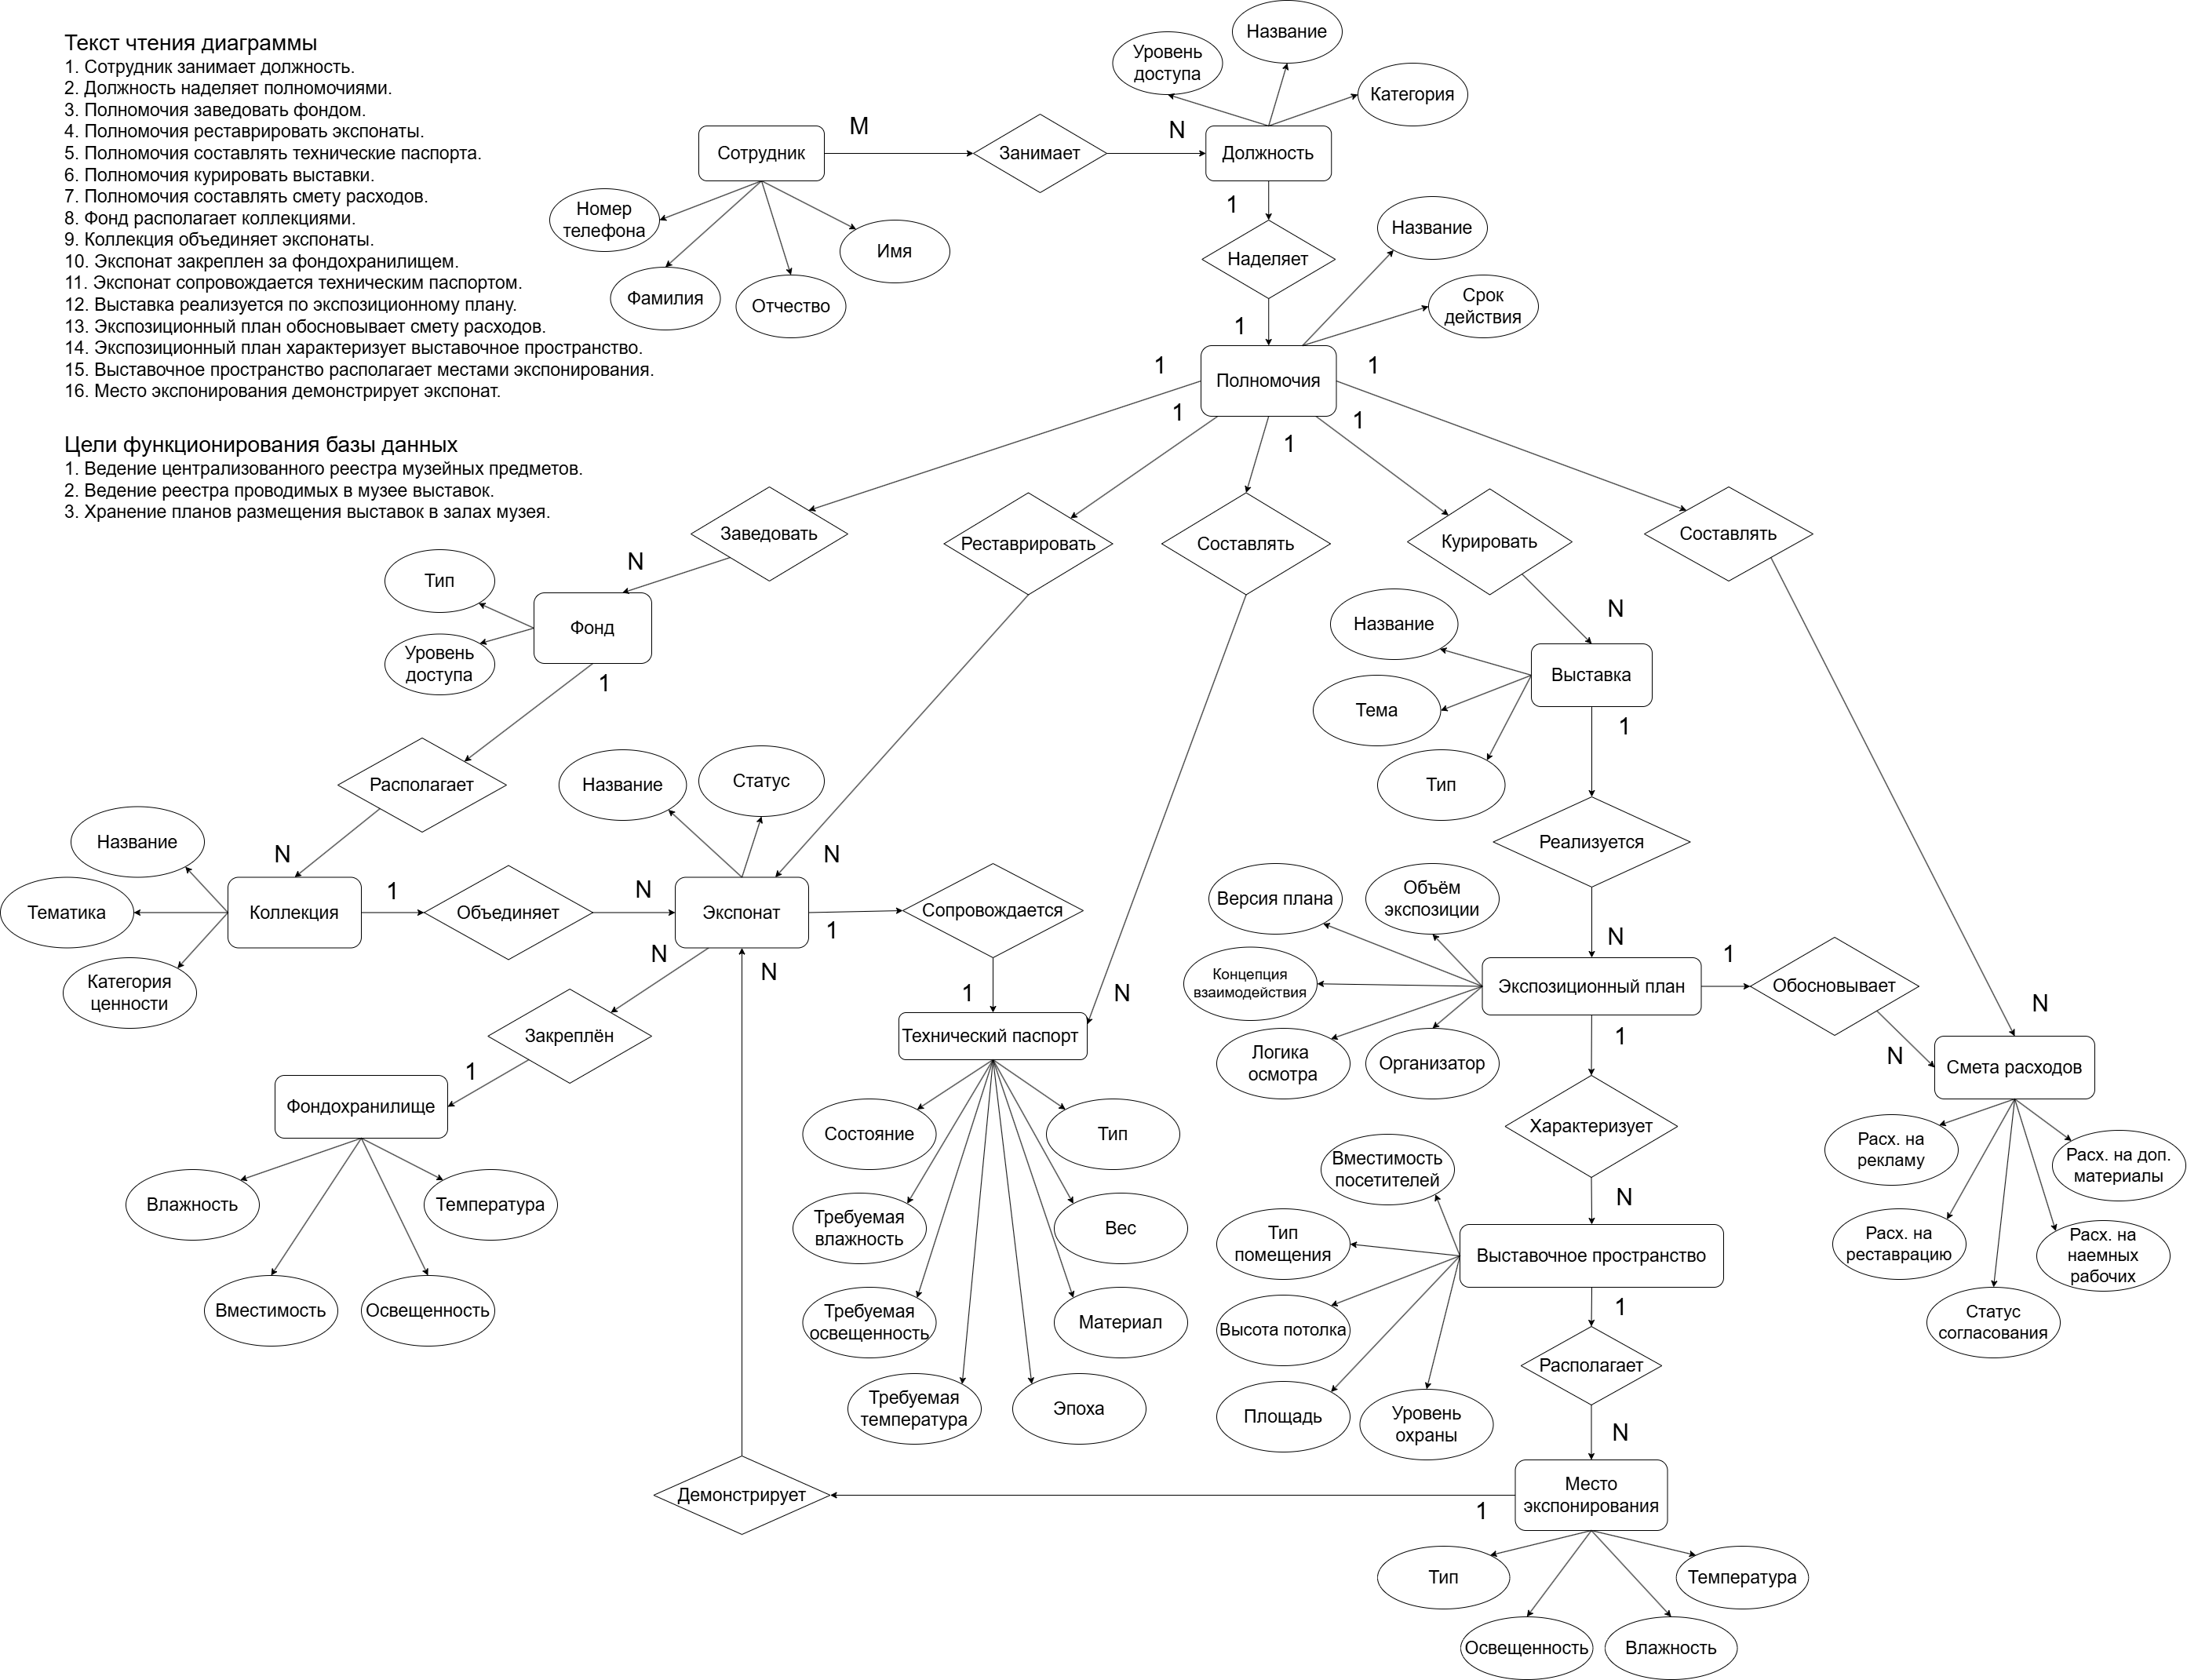
\includegraphics[height=24cm]{pic/ER версия 2.png}
    \caption{ER-диаграмма}
    \label{ER}
\end{figure}

\clearpage
\MySavedValues
\recalctypearea

\newpage


Схема связи объектов представлена на Рис.\ref{objects_shema}.

\begin{figure}[H]
    \centering
    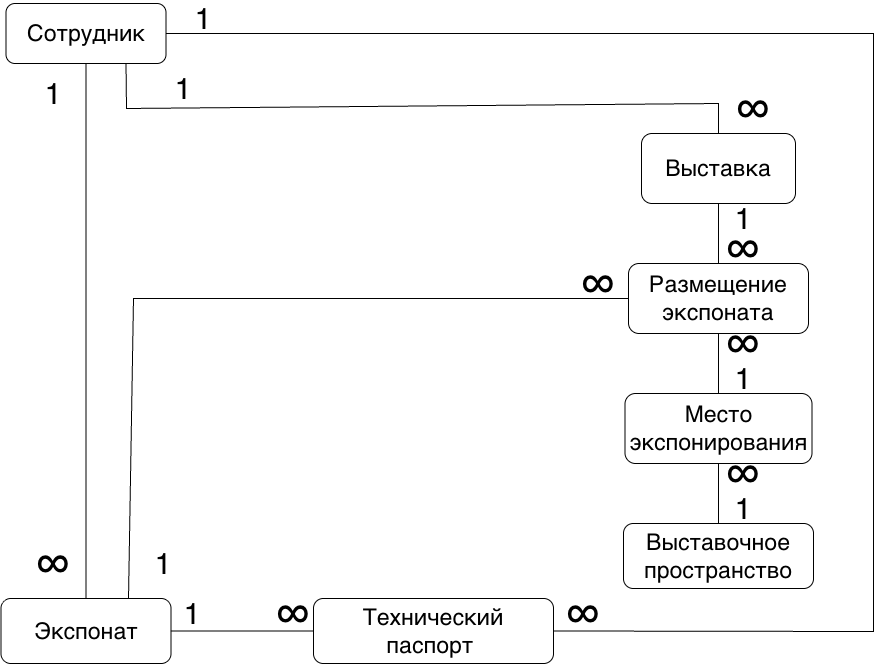
\includegraphics[height=10cm]{pic/Иерархия сокращенная.png}
    \caption{Схема связи объектов}
    \label{objects_shema}
\end{figure}


\begin{enumerate}
    \item Один сотрудник может курировать множество выставок (1 - $\infty$).
    \item За одним сотрудником может быть закреплено много экспонатов (1 - $\infty$).
    \item Один сотрудник может составить много технических паспортов (1 - $\infty$).
    \item Одно выставочное пространство включает в себя множество конкретных мест экспонирования (стендов, витрин) (1 - $\infty$).
    \item В рамках одной выставки выставляется множество экспонатов в местах экспонирования (размещение экспоната) (1 - $\infty$).
    \item Одно место экспонирования может быть связано с множеством записей о размещении экспонатов (разные предметы в разное время) (1 - $\infty$).
    \item Один экспонат может иметь разные версии технических паспортов (1 - $\infty$).
    \item Один экспонат может быть размещен в разных местах экспонирования на разных выставках (размещение экспоната) (1 - $\infty$).
\end{enumerate}